\documentclass[12pt,american,final, a4paper]{memoir}
\usepackage{csquotes}
\usepackage{babel}
\usepackage{enumitem}
\usepackage{geometry}
\usepackage{booktabs}
\usepackage{xparse}
\makeatletter
\let\afhead\@afterheading% For use with etoc
\makeatother
\usepackage{etoc}
\usepackage{float}
\usepackage[T1]{fontenc}
\usepackage[babel,final,tracking=true,kerning=true,spacing=true,activate={true,nocompatibility}]{microtype}
\usepackage{graphicx}
\usepackage[all]{nowidow}  % avoids widow lines at all costs
\doublehyphendemerits=100000 % and hyphens on successive lines
\usepackage{newpxtext,textcomp}
\usepackage{mathtools,amssymb}
\usepackage[euler-hat-accent]{eulervm}
\usepackage[cal=euler,frak=euler,bb=boondox,scr=boondoxupr]{mathalpha}
\usepackage[type1]{cabin}
\usepackage[varqu,varl]{inconsolata}
\usepackage[backend=biber,style=alphabetic]{biblatex}
\addbibresource{sample.bib}
\usepackage[hypcap=true]{caption} % Anchors links to the beginning of their respective floats. Load after hyperref.
\usepackage[pdfencoding=auto,pdfborderstyle={/S/U/W 1}]{hyperref} % Clickable references.
\usepackage[noabbrev,nameinlink]{cleveref} % Names references automatically. Load after hyperref.
\usepackage{nameref}
\hypersetup{pdfprintscaling=None}
\usepackage[section]{placeins}
\makeatletter
\AtBeginDocument{%
  \expandafter\renewcommand\expandafter\subsection\expandafter{%
    \expandafter\@fb@secFB\subsection
  }%
}
\makeatother%
\usepackage{geometry}
\usepackage{algorithmicx}
\usepackage[ruled]{algorithm}
\usepackage{algpseudocode}
%\usepackage[dvipsnames]{xcolor}
\usepackage[amsmath,hyperref,thmmarks]{ntheorem}
\usepackage{thmtools}
\usepackage{todonotes}
\presetkeys{todonotes}{inline}{} % inline todos
\ExplSyntaxOn
\DeclareExpandableDocumentCommand{\IfNoValueOrEmptyTF}{mmm}
 {
  \IfNoValueTF{#1}{#2}
   {
    \tl_if_empty:nTF {#1} {#2} {#3}
   }
 }
\ExplSyntaxOff

\usetikzlibrary{automata,positioning}
%\setlist{nosep} % or \setlist{noitemsep} to leave space around whole list
\setlist{noitemsep}

% this is for CFGs
\usepackage{listings}
\lstset{columns=fullflexible,
  mathescape=true,
  xleftmargin=.25\textwidth,
  literate={->}{\ensuremath{\rightarrow{}}}{1}
  {=>}{\ensuremath{\mskip\medmuskip\Rightarrow{}}}{1}
  {|}{\ensuremath{\mathbin{}\mskip\medmuskip\vert\mskip\medmuskip}}{1}
  {a}{\ensuremath{a}}{1}
  {b}{\ensuremath{b}}{1}
  {c}{\ensuremath{c}}{1}
  {d}{\ensuremath{d}}{1}
  {e}{\ensuremath{e}}{1}
  {f}{\ensuremath{f}}{1}
  {g}{\ensuremath{g}}{1}
  {h}{\ensuremath{h}}{1}
  {i}{\ensuremath{i}}{1}
  {j}{\ensuremath{j}}{1}
  {k}{\ensuremath{k}}{1}
  {l}{\ensuremath{l}}{1}
  {m}{\ensuremath{m}}{1}
  {n}{\ensuremath{n}}{1}
  {o}{\ensuremath{o}}{1}
  {p}{\ensuremath{p}}{1}
  {q}{\ensuremath{q}}{1}
  {r}{\ensuremath{r}}{1}
  {s}{\ensuremath{s}}{1}
  {t}{\ensuremath{t}}{1}
  {u}{\ensuremath{u}}{1}
  {v}{\ensuremath{v}}{1}
  {w}{\ensuremath{w}}{1}
  {x}{\ensuremath{x}}{1}
  {y}{\ensuremath{y}}{1}
  {z}{\ensuremath{z}}{1}
  {A}{\ensuremath{A}}{1}
  {B}{\ensuremath{B}}{1}
  {C}{\ensuremath{C}}{1}
  {D}{\ensuremath{D}}{1}
  {E}{\ensuremath{E}}{1}
  {F}{\ensuremath{F}}{1}
  {G}{\ensuremath{G}}{1}
  {H}{\ensuremath{H}}{1}
  {I}{\ensuremath{I}}{1}
  {J}{\ensuremath{J}}{1}
  {K}{\ensuremath{K}}{1}
  {L}{\ensuremath{L}}{1}
  {M}{\ensuremath{M}}{1}
  {N}{\ensuremath{N}}{1}
  {O}{\ensuremath{O}}{1}
  {P}{\ensuremath{P}}{1}
  {Q}{\ensuremath{Q}}{1}
  {R}{\ensuremath{R}}{1}
  {S}{\ensuremath{S}}{1}
  {T}{\ensuremath{T}}{1}
  {U}{\ensuremath{U}}{1}
  {V}{\ensuremath{V}}{1}
  {W}{\ensuremath{W}}{1}
  {X}{\ensuremath{X}}{1}
  {Y}{\ensuremath{Y}}{1}
  {Z}{\ensuremath{Z}}{1}
}
\theoremstyle{plain}

\usepackage{mdframed} % for boxing thingys
\newmdtheoremenv[
outerlinewidth=2,leftmargin=40,%
rightmargin=40,backgroundcolor=yellow,%
outerlinecolor=blue,innertopmargin=0pt,%
splittopskip=\topskip,skipbelow=\baselineskip,%
skipabove=\baselineskip,ntheorem
]{theorem}{Theorem}

\newmdtheoremenv{definition}{Definition}
\newmdtheoremenv{corollary}{Corollary}
\newtheorem{claim}{Claim}
\theorembodyfont{\upshape}
\theoremheaderfont{\scshape\bfseries}
\newtheorem{prob}{Problem}
\crefname{prob}{problem}{problems}
\Crefname{prob}{Problem}{Problems}
\theoremstyle{nonumberplain}
\newtheorem{proof}{Proof}
% Proof environment for induction
\newenvironment{proofmathinduction}[1][\proofname]
{
	\begin{proof}[\textbf{\textup{Proof by Mathematical Induction}} on #1.]$ $\par\nobreak\ignorespaces
}{%
	\end{proof}
}

\newenvironment{proofstructuralinduction}[1][\proofname]
{
	\begin{proof}[\textbf{\textup{Proof by Structural Induction}}]$ $\par\nobreak\ignorespaces
	}{%
	\end{proof}
}

\NewDocumentCommand{\problem}{ommm}{%
  \IfNoValueOrEmptyTF{#1}{\begin{prob}[#2]\quitvmode}{\begin{prob}[#1]{\scshape\bfseries#2}\label{prob:#1}}
  \begin{itemize}
	\item[\textsc{Instance:}] #3
	\item[\textsc{Question:}] #4
  \end{itemize}
  \end{prob}
}

\newcommand{\FA}{\textsf{FA}}
\newcommand{\DFA}{\textsf{DFA}}
\newcommand{\NFA}{\textsf{NFA}}

\newcommand{\setofstatesname}{S}
\newcommand{\startstatename}{s_0}
\newcommand{\acceptstatesname}{A}
\newcommand{\transitionfunctionname}{\delta}
\newcommand{\inputalphabetname}{\Sigma}
\newcommand{\stackalphabetname}{\Gamma}
\newcommand{\tapealphabetname}{\Gamma}
\newcommand{\blanksymbol}{\sqcup}

\newcommand{\Pcomplexity}{\textsf{P}}
\newcommand{\NP}{\textsf{NP}}

\newcommand{\natnums}{\mathbb{N}}
\newcommand{\integers}{\mathbb{N}}
\newcommand{\reals}{\mathbb{R}}

\newcommand{\union}{\cup}
\newcommand{\concat}{\circ}
\newcommand{\orop}{|}
\renewcommand{\complement}[1]{\overline{#1}}
\newcommand{\emptystring}{\varepsilon}

\newcommand{\Epsilon}{\varepsilon}

\newcommand{\powerset}[1]{\mathcal{P}(#1)}

\newcommand{\includecontent}[1]{\input{content/#1}}
% Force floats in right section.
%\chapterstyle{bianchi}
%\chapterstyle{ger}
\chapterstyle{ell}
\cftsetindents{part}{0em}{1.65em} % accommodate for part numbers (add some space)
\let\originalchapter\chapter%
\RenewDocumentCommand{\chapter}{som}{%
  \IfBooleanTF{#1}
    {\originalchapter*{#3}}
    {\IfNoValueTF{#2}
      {\originalchapter{#3}}
      {\originalchapter[#2]{#3}}%
    }% Manage chapter like normal command
\etocchecksemptiness% Check if ToC is empty if so, do nothing
\etocsettocstyle{% style before the chapter's ToC
\microtypesetup{protrusion=false}% Disable microtype for ToCs
\noindent\hrulefill\large\bfseries% Traces the line before Contents
\kern2ptContents\kern2pt\hrulefill% Spaces & line after Contents
\vspace{0.5\onelineskip}% Space below the top line
}
{%style after the chapter's ToC
\noindent\hrulefill% Trace the line below ToC
\par\nobreak\addvspace{\midchapskip}% Add spaces if needed
\afhead% Warn TeX engine we are after a heading (without effect if ToC empty, duplicate)
\microtypesetup{protrusion=false}% Re-enable microtype
}
\localtableofcontents\afhead\microtypesetup{protrusion=true}}% print the local ToC and setup like @afterheading
\etocsettocdepth{subsection} % chapters, sections, and subsections are in the Table of Contents

%%%---%%%---%%%---%%%---%%%---%%%---%%%---%%%---%%%---%%%---%%%---%%%---%%%

\setlrmarginsandblock{0.15\paperwidth}{*}{1} % Left and right margin
\setulmarginsandblock{0.15\paperwidth}{*}{1}  % Upper and lower margin
\setheaderspaces{*}{*}{1}

\checkandfixthelayout
 \pretitle{\vspace{0.1\paperwidth}\begin{center}\Huge\bfseries}
 \posttitle{\par\vfill\end{center}}
\predate{\vfill\begin{center}\large}
\showboxdepth=\maxdimen
\showboxbreadth=\maxdimen

\title{Easy Theory of Computation}
\author{Ryan E. Dougherty}
\date{}


\begin{document}

\hypersetup{pageanchor=false}% don't try to anchor on unnumbered pages & roman numbers
\begin{titlingpage}
\sffamily
\maketitle
\end{titlingpage}
\frontmatter
%%%---%%%---%%%---%%%---%%%---%%%---%%%---%%%---%%%---%%%---%%%---%%---%%%
%%%---%%%---%%%---%%%---%%%---%%%---%%%---%%%---%%%---%%%---%%%---%%%---%%%
\microtypesetup{protrusion=false}% protrusion may lead to  leaders dots issues in TOCs. Disabling it for now
\tableofcontents
\microtypesetup{protrusion=true}
\mainmatter\hypersetup{pageanchor=true}%
%\part{Introduction}
%\chapter{Introduction and Review: Logic, Proofs, Sets, and Functions, Relations, and Regular Expressions}

\section{Objectives}

\begin{itemize}
	\item Describe and apply basic operations of logic.
	\item Describe and apply basic operations of set theory (and languages as sets of strings).
	\item Define the properties of functions and equivalence relations.
	\item Review and practice reading and writing regular expressions.
\end{itemize}

\section{Introduction + Motivation}

\section{Definitions}

Some common sets are the \emph{natural numbers} $\natnums$, which are the numbers $0, 1, 2, 3, \cdots$; the \emph{integers} $\integers$, which are the numbers $\cdots, -3, -2, -1, 0, 1, 2, 3, \cdots$; and the \emph{real numbers} $\reals$.

A \emph{set} is a collection of ``elements'' without duplicates, usually written with curly braces and not in any particular order, like: \{3, 4, 2, ``New York''\}.
If $A$ and $B$ are two sets, then the notation $A \subseteq B$ indicates that $A$ is a \emph{subset} of $B$, in that every element of the set $A$ is also in the set $B$. An example is $A = \{0, 1, 4\}$ and $B = \{0, 1, 4, 7\}$.
If $A \subseteq B$ and some element of $B$ is also not in $A$, $A$ is a \emph{proper} subset of $B$, written $A \subset B$ (and the previous example shows that $A$ is a proper subset of $B$).
The set with no elements is called the \emph{empty set}, written $\emptyset$.

If $A$ is a set, then $\powerset{A}$ is the \emph{power set} of $A$, which is the collection of all subsets of $A$, including $A$ itself.

\section{Examples}

\section{Problems}

\begin{enumerate}
	\item Let $L = \{a, b, c\}$; compute the set $LL$.
	\item Let $L = \{0, 1, 2, 3, 4, 5, 6, 7, 8, 9\}$; describe the language $L^+$ in English.
	\item For each of the functions below, indicate which of the properties hold: total, one-to-one, onto, and/or bijection.
	\begin{enumerate}
		\item $m: \natnums \to \natnums$ defined by $m(x) = \min(x, 2)$.
		\item $s: \natnums \to \reals$ defined by $s(x) = \sqrt{x}$.
		\item $d: \natnums \to \reals$ defined by $d(x) = \frac{1}{x}$.
		\item $i: \natnums \to \natnums$ defined by $i(x) = x$.
		\item $c: \reals^{0+} \to \natnums$ defined by $c(x) = \lceil x \rceil$, where $\reals^{0+}$ indicates non-negative real numbers.
		\item $e: \natnums \to \natnums$ defined by $e(x) = 2x$.
		\item $f: \natnums \to \integers$ defined by:
		\[
			f(x) = 
			\begin{cases}
				\frac{x}{2},& \text{if $x$ is even}\\
				\frac{-x-1}{2},& \text{otherwise}
			\end{cases}
		\]
	\end{enumerate}
	
	\item For the following languages, show a corresponding regular expression.
	\begin{enumerate}
		\item All strings in $\{0,1\}^\star$ containing exactly two 0's.
		\item All strings in $\{0,1\}^\star$ containing at least two 0's.
		\item All strings in $\{0,1\}^\star$ that do not end in 01.
	\end{enumerate}

	\item  In each case below, find a string of minimum length in $\{a, b\}^\star$ not in the language corresponding to the given regular expression.
	\begin{enumerate}
		\item $b^\star (ab)^\star a^\star$
		\item $(a^\star \orop b^\star)(a^\star \orop b^\star)(a^\star \orop b^\star)$
		\item $a^\star (baa^\star)^\star b^\star$
		\item $b^\star (a \orop ba)^\star b^\star$
	\end{enumerate}
\end{enumerate}
%\chapter{Recursive Definitions and Proof by Induction}

\section{Objectives}

\begin{itemize}
	\item Know the terminology and operations of Languages.
	\item Describe the elements of a recursive definition.
	\item Define languages recursively.
	\item Know the basic elements of a proof by induction.
	\item Prove properties using induction.
\end{itemize}

\section{Introduction + Motivation}

Many structures we will analyze in this course have a ``simple'' structure, in that they are one of a small number of possibilities. 
Many functions you may have come across have such a simple structure; here are a few:
%\[
%	fib(n) = \begin{cases}
%		1 & \text{if $n = 0, 1$}\\
%		fib(n-1) + fib(n-2) & \text{if $n > 1$}
%	\end{cases}
%\]
The ``fibonacci'' function $fib: \natnums \to \natnums$ defined by:
\[
fib(n) = 
\begin{cases}
	1 & \text{if $n=0, 1$}\\
	fib(n-1) + fib(n-2) & \text{if $n > 1$}
\end{cases}
\]

The ``factorial'' function $!: \natnums \to \natnums$ defined by:
\[
n! = 
\begin{cases}
	1 & \text{if $n=0$}\\
	n \times (n-1)! & \text{if $n > 1$}
\end{cases}
\]

``Reversing'' a single string $reverse: \Sigma^\star \to \Sigma^\star$ defined by:
\[
reverse(s) = 
\begin{cases}
	s & \text{if $|s| \le 1$}\\
	s(n) \concat reverse(s(1..(n-1))) & \text{otherwise}
\end{cases}
\]
where $s$ is a string of length $n$, and $s(i..j)$ represents the substring from index $i$ to $j$.

\section{Recursive Definitions}

Note that in all of the examples above, they all have the same essential ``structure'':
\begin{itemize}
	\item One or more \emph{basis parts} that define a finite number of elements in the set.
	\item One or more \emph{recursive parts} that produce new elements in the set, given known existing elements.
	\item A \emph{closure} statement that removes any ambiguity of other elements potentially being in the set.\footnote{In the examples given earlier, the domain/codomain of the function implicitly give the necessary closure statement.}
\end{itemize}

\section{Mathematical Induction Review}

The general method for proving a statement by induction involves the following steps:
\begin{enumerate}
	\item Write down the claim you are trying to prove; be sure to always state the claim!
	
	What to write: 
	\begin{mdframed}[align=center]
		\textbf{Claim: $\langle$ write the actual formal statement of the claim here $\rangle$}
	\end{mdframed}

	\item Indicate what proof style you are using (which is induction in this case).
	
	What to write: 
	\begin{mdframed}[align=center]
		\textbf{Proof by Induction on $\langle$ some variable(s) here $\rangle$}
	\end{mdframed}

	\item What is/are the base case(s), followed by a proof of each. 
	
	What to write: 
	\begin{mdframed}[align=center]
		\textbf{Base Case 1 $\langle$ set the variable(s) to the first base case value(s) $\rangle$}:\\ $\langle$ proof that the claim holds for this first base case $\rangle$.\\
		$\cdots$\\
		\textbf{Base Case $m$ $\langle$ set the variable(s) to the $m$th base case value(s) $\rangle$}: \\$\langle$ proof that the claim holds for this $m$th base case $\rangle$.
	\end{mdframed}
	
	\item Induction Hypothesis statement, indicating what you assume about some variable(s).
	
	What to write:
	\begin{mdframed}[align=center]
		\textbf{Induction Hypothesis}: Assume that for $\langle$ variable + domain excluding base case(s) $\rangle$ that the claim is correct.
	\end{mdframed}

	\item Induction Step, which is the next ``largest'' value for the variable(s) indicated in the Induction Hypothesis statement.
	
	What to write:
	\begin{mdframed}[align=center]
		\textbf{Induction Step ($\langle$ next largest domain for the variable(s) $\rangle$)}: $\langle$ proof that the claim is true in this case using the Induction Hypothesis \emph{explicitly} $\rangle$.
	\end{mdframed}

	\item Concluding statement.
	
	What to write:
	\begin{mdframed}[align=center]
		\textbf{Conclusion}: By the principle of $\langle$ the type of induction used $\rangle$ induction, it follows that $\langle$ restate the claim here $\rangle$.
	\end{mdframed}
	
\end{enumerate}

Let's do an example, using \emph{mathematical} induction. The function $n!$ is strictly larger than $2^n$ for all integers $n \ge 4$.

\begin{claim*}
	$n! > 2^n$ for all $n \ge 4$.
\end{claim*}

\begin{proofmathinduction}[$n \ge 4$]

	\textbf{Base Case $(n = 4)$}: We must show that $4! > 2^4$. By definition of factorial, $4! = 4 \cdot 3 \cdot 2 \cdot 1 = 24$, and $2^4 = 16$. Since $24 > 16$, this claim holds for this base case.
	
	\textbf{Induction Hypothesis}: Assume that for \emph{some}\footnote{Note this says \emph{some} and not \emph{all}. If we said \emph{all}, we would be assuming the claim to be true before proving it!} $n \ge 4$, $n! > 2^n$.
	
	\textbf{Induction Step $(n + 1)$}: We must show that $(n+1)! > 2^{n+1}$. Starting with the left-hand side,\footnote{We must only manipulate one side of the equation in order to prove this. You are \textbf{not} allowed to manipulate both sides of the equation at the same time!}
	\begin{alignat*}{3}
		&(n+1)! &&= (n+1) \cdot n! \quad && \text{By Definition of Factorial} \\
		& 		&&> (n+1) \cdot 2^n \quad&& \text{By the Induction Hypothesis} \\
		& 		&&> 2 \cdot 2^n \quad&& \text{Since $n \ge 4$} \\
		&		&&= 2^{n+1} \quad&& \text{By Definition of $2^{n+1}$}
 	\end{alignat*}
 	It follows that $(n+1)! > 2^{n+1}$, which is what we wanted to prove.
 	
 	\textbf{Conclusion}: By the principle of mathematical induction, it follows that $n! > 2^n$ for all $n \ge 4$.
\end{proofmathinduction}

\section{Problems}

\begin{enumerate}
	\item (AY15-1 WPR Question) Give a recursive definition for each of the following sets.
	\begin{enumerate}
		\item The set $W$ of all strings of the form $1^i 0^k$ where $i \ge 2k$.
		\item The set $X$ of all strings in $\{0,1\}^\star$ containing the substring 00.
		\item The set $Y$ of all strings over $\Sigma = \{0,1\}$ that contain more 0s than 1s.
	\end{enumerate}

	\item (AY16-2 WPR Question) Give a recursive definition for each of the following sets.
	\begin{enumerate}
		\item The set $B$ of all strings in $\{0,1\}^\star$ containing the substring 101101.
		\item The set $C$ of all strings of rhe form $1^x 01^j$, where $j \le x \le 2j$. 
	\end{enumerate}
	
	\item Let $f(0) = 1, f(n) = 2f(n-1)+1$ for all $n > 0$.
	Prove by induction that for any $n \ge 0$, $f(n) = 2^{n+1} - 1$.
	
	\item Prove using mathematical induction that for every $n \in \natnums$,
	\[
		1 + \sum_{i=1}^{n} i \times i! = (n+1)!.
	\]
	
	\item Let $f_i$ be the $i$th Fibonacci number (i.e., $f_0 = 0, f_1 = 1$, and for $n \ge 2$, $f_n = f_{n-1} + f_{n-2}$).
	Prove by mathematical induction that:
	\[
		\sum_{i=1}^{n} f_i = f_{n+2} - 1.
	\]
	
	\item Suppose $x$ is any real number greater than $-1$. Prove using mathematical induction that for every nonnegative integer $n$, $(1+x)^n\ge1+nx$. (Be sure you say in your proof exactly how you use the assumption that $x>-1$.
	
	\todo{Add other exercises}
\end{enumerate}
%\chapter{Structural Induction}

\section{Objectives}

\begin{itemize}
	\item Describe the essential components of a proof by structural induction.
	\item Prove properties using structural induction.
\end{itemize}

\section{Introduction + Motivation}

Structural induction is an inductive proof technique that uses the structure (recursive definition or nature) of the elements in a set to prove a property about that set.  The steps to do this are very similar to those used for mathematical induction.

Suppose $L$ is defined recursively and you want to prove that every element $x \in L$ has property $P$.  Then you can prove your claim as done in the following section.


\section{Structural Induction}

The general method for proving a statement by structural induction involves the following steps (items that are bolded are different than mathematical induction):
\begin{enumerate}
	\item Write down the claim you are trying to prove; be sure to always state the claim!
	
	\item Indicate what proof style you are using (which is \textbf{structural} induction in this case).
	
	What to write: 
	\begin{mdframed}[align=center]
		\textbf{Proof by Structural Induction} (no variables this time)
	\end{mdframed}
	
	\item What is/are the base case(s), followed by a proof of each. 
	
	What to write: 
	\begin{mdframed}[align=center]
		Base Case 1 $\langle$ \textbf{some element} $\rangle$:\\ $\langle$ proof that this element has property $P$ $\rangle$.\\
		$\cdots$\\
		Base Case 1 $\langle$ \textbf{some element} $\rangle$:\\ $\langle$ proof that this element has property $P$ $\rangle$.\\
	\end{mdframed}
	
	\item Induction Hypothesis statement, indicating what you assume about some variable(s).
	
	What to write:
	\begin{mdframed}[align=center]
		\textbf{Induction Hypothesis}: Assume that $\langle$ \textbf{some variable in the set $L$} $\rangle$ \textbf{has the property $P$}.
	\end{mdframed}
	
	\item Induction Step, \textbf{proving that recursively constructed elements in the rules also have property $P$}
	
	What to write:
	\begin{mdframed}[align=center]
		Induction Step ($\langle$ \textbf{one recursively defined element} $\rangle$): $\langle$ \textbf{proof that this element also has property $P$} using the Induction Hypothesis \emph{explicitly} $\rangle$.
	\end{mdframed}
	
	\item Concluding statement.
	
\end{enumerate}

Let's do an example, using \emph{structural} induction.
Let $L$ be a subset of $\Sigma = \{a,b\}$ be the language defined as follows:
\begin{enumerate}
	\item $\emptystring \in L$.
	\item For any $x \in L$, $axb \in L$.
	\item No string is in $L$ unless it can be obtained from rules 1, 2.
\end{enumerate}

\begin{claim}
Every element in $L$ is even in length.
\end{claim}

\begin{proofstructuralinduction}

	\textbf{Base Case} ($\emptystring$): We must show that all elements defined in the basis rules are even in length. Thus, we must show that $\emptystring$ is even in length. Since $|\emptystring| = 0$, and 0 is even, the property holds for the basis.
	
	\textbf{Induction Hypothesis}: Assume $x \in L$ is a string that is even in length.
	
	\textbf{Induction Step ($axb$)}: We must show that the elements constructed in the recursive rules are even in length.
	Thus, we must show that $axb$ is even in length.
	\begin{itemize}
		\item $|axb| = 1 + |x| + 1 = 2 + |x|$.
		\item By the induction hypothesis, $|x| = 2k$ for some integer $k$.
		\item It follows that $|axb| = 2 + 2k$.
		\item Since $2+2k$ is even, $|axb|$ is even, and the property thus holds for the recursive rules.
	\end{itemize}

	\item Conclusion: Since every element in $L$ can be constructed using a finite number of applications of rules 1 and 2 and we have proven that rules 1 and 2 maintain the property of even-in-length, all strings in $L$ are even in length.
	
\end{proofstructuralinduction}



\section{Examples}

\section{Problems}
\part{Regular Languages}
\chapter{Finite Automata}

\section{Objectives}

\begin{itemize}
	\item Define finite automata.
	\item Interpret (``read'') finite automata that are a language acceptors.
	\item Design (``write'') finite automata that are a language acceptors.
	\item Design finite automata to accept the union, intersection, and difference of two languages.
\end{itemize}

\section{Introduction + Motivation}

\section{Definitions}

\begin{minipage}{.7\linewidth}
	A \textit{finite automaton} (\FA) consists of 5 parts:
\begin{itemize}
	\item $\setofstatesname$, a finite set of \textit{states};
	\item $\startstatename$, a state in $\setofstatesname$ called the \textit{start state};
	\item $\acceptstatesname$, a subset of $\setofstatesname$ called the \textit{accept states};
	\item $\inputalphabetname$, a finite set, called the \textit{input alphabet};
	\item $\transitionfunctionname$, a function from $\setofstatesname \times \inputalphabetname$ to $\setofstatesname$, called the \textit{transition function}.
\end{itemize}

\end{minipage}
\hfill
\begin{minipage}{.3\linewidth}
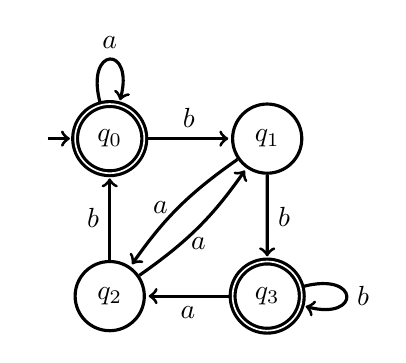
\begin{tikzpicture}[scale=0.7, shorten >=1pt,node distance=2cm,on grid,auto,initial text={},every state/.style={align=center},line width=0.4mm] 
	\node[state,initial,accepting,inner sep=5pt] (q_0)   {$q_0$}; 
	\node[state] (q_1) [right=of q_0] {$q_1$}; 
	\node[state] (q_2) [below=of q_0] {$q_2$}; 
	\node[state,accepting,inner sep=5pt](q_3) [below=of q_1] {$q_3$};
	\path[->] 
	(q_0) edge [loop above] node {$a$} ()
	edge  [] node {$b$} (q_1)
	(q_1) edge  [bend right=10, left] node {$a$} (q_2)
	edge [] node {$b$} (q_3)
	(q_2) edge [] node {$b$} (q_0) 
	edge [bend right=10,below] node {$a$} (q_1)
	(q_3) edge [loop right] node {$b$} () 
	edge [] node {$a$} (q_2);
\end{tikzpicture}
\end{minipage}

A finite automaton is called \textit{deterministic} if the transition function $\transitionfunctionname$ is a \textit{total} function (i.e., every input to $\transitionfunctionname$ has a defined output); we call this a \textit{deterministic finite automaton}, or \DFA.

\subsection{$\DFA$ Computations}

Let $M$ be a $\DFA$, and $w \in \inputalphabetname^\star$. Informally, $M$ accepts $w$ if the state that $M$ goes into on input $w$ is any accept state.
Formally, let the \textit{computation of $M$ on $w$} is the sequence of states $s_1, s_2, \cdots, s_n, s_{n+1}$ where $w = w_1 \cdots w_n$ with $w_i \in \Sigma$ such that $\delta(s_i, w_i) = s_{i+1}$ for all $1 \le i \le n$.
Such a computation is \textit{accepting} if $s_{n+1}$ is an accept state (i.e., $s_{n+1} \in \acceptstatesname$).

Note in the definition here we said that $M$'s computation on $w$, implying $M$ has exactly one computation on $w$, but we haven't actually proven this yet; let's do this.

\begin{claim*}
	Every $\DFA$ $M$ has exactly one computation on any string $w \in \inputalphabetname^\star$, where $\inputalphabetname$ is the input alphabet of $M$.
\end{claim*}

\begin{proofstructuralinduction}[$|w|$]
	\item \textbf{Base Case} ($w = \emptystring$): We must show that all elements defined in the basis rules have that $M$ has exactly one computation on them. Thus, we must show that $M$ has exactly one computation on $w = \emptystring$. 
	
	Note that $|w| = |\emptystring| = 0$. Since the input has no characters to read, no transitions can be applied. Therefore, the computation of $M$ on $\emptystring$ is $(q_0)$, where $q_0$ is the start state of $M$.
	Since this is the only possible sequence of states, $M$ has exactly 1 computation on $\emptystring$.
	
	\item \textbf{Induction Hypothesis}: Assume any string $w \in \inputalphabetname^\star$ with $|w| \le k$ for some integer $k$ has that $M$ has exactly 1 computation on $w$.
	
	\item \textbf{Induction Step ($k+1$)}: We must show that any string of length $k+1$ in $\inputalphabetname^\star$ has this property.
	Call such a string $w'$. 
	By definition, $w'$ must be equal to $wa$, where $a \in \inputalphabetname$, and $w \in \inputalphabetname^\star$ with $|w| = k$.
	By the Induction Hypothesis, $M$ has exactly 1 computation on $w$; call that sequence of states $(q_0, q_1, \cdots, q_k)$.
	Denote $q_{k+1} = \transitionfunctionname(q_k, a)$, where $\transitionfunctionname$ is the transition function of $M$.
	This state is defined because $M$ is a $\DFA$, and so the computation of $M$ on $w'$ must include $q_0, \cdots, q_k, q_{k+1}$.
	Since the transition function $\transitionfunctionname$ is only a function, $q_{k+1}$ is uniquely determined. 
	Therefore, $M$ has exactly one computation on $w'$; namely, $(q_0, \cdots, q_k, q_{k+1})$.
	
	\item \textbf{Conclusion}: Since $M$ has exactly one computation on every string in $\inputalphabetname^\star$, and $M$ is an arbitrary $\DFA$, we have proven that every $\DFA$ has exactly one computation on every string in $\inputalphabetname^\star$.
\end{proofstructuralinduction}

Note that the Induction Step shows that if $M$ is merely an $\FA$ instead of a $\DFA$, $M$ might not read the whole string $w'$, since $\transitionfunctionname(q_k, a)$ may not be defined.
This does show that $\FA$s have either \emph{0 or 1} computations on every string.

The \textit{language} of a $\DFA$ $M$, written $L(M)$, is the set of all strings $w \in \inputalphabetname^\star$ that $M$ accepts. Formally,
\[
	L(M) = \{ w \in \inputalphabetname^\star : \text{$M$'s computation on $w$ is accepting}\}
\]



\section{Examples}

\todo{Unary multiples of n}

\todo{Binary multiples of n}

\section{Problems}
\chapter{DFA Minimization}

\section{Objectives}

\begin{itemize}
	\item Apply the minimization algorithm to finite automata.
\end{itemize}

\section{Introduction + Motivation}

We want to minimize the size of a finite automaton as much as possible, \emph{as long as it has the same language as that of the original.}

\section{Minimization}

Think about the following two states:

\todo{fix the transition labels and state names}
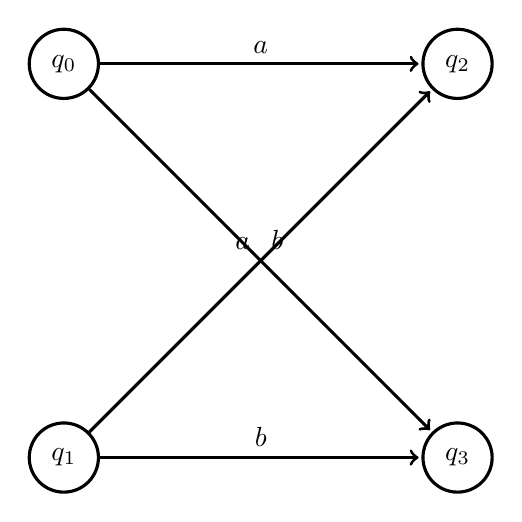
\begin{tikzpicture}[scale=0.7, shorten >=1pt,node distance=5cm,on grid,auto,initial text={},every state/.style={align=center},line width=0.4mm] 
	\node[state] (q_0)   {$q_0$}; 
	\node[state] (q_1) [below=of q_0] {$q_1$}; 
	\node[state] (q_2) [right=of q_0] {$q_2$}; 
	\node[state] (q_3) [below=of q_2] {$q_3$}; 
	\path[->] 
	(q_0) edge node {$a$} (q_2)
	(q_0) edge node {$b$} (q_3)
	(q_1) edge node {$a$} (q_2)
	(q_1) edge node {$b$} (q_3)
	;
\end{tikzpicture}

Clearly these two states ``do the same thing,'' since their transitions go to identically the same states, given the same input from both.
Here, we can just merge the two states together:

\todo{Same example, one state on the left with the name containing the original two}

However, it may be more complicated to  figure out, say, this example of what states are the ``same'':

\todo{Bigger example}

One attempt to minimize an automaton $M$ is to try all ``smaller'' automata $m$, and check if the languages of $M$ and $m$ are the same.
Several problems arise: if $M$ is moderately big, the number of automata smaller than it is \emph{enormous}.
Setting that aside, how would one check  if $M$ and $m$ have the same language, in general? Note that $M, m$ have to accept the same strings, \emph{and not accept} the same strings.
If you have a small example of $M, m$ in front of you, maybe that can be done by inferring some properties of both. 
But in general, how would that be done? Checking all infinitely many strings against both machines clearly will take too long, so we need a better idea.

\subsection{Distinguishing States}

Instead of thinking about two states $p, q$ and reading a single character, let's think about \emph{every possible string that can be read from $p, q$}.
If, for \emph{any} string $w \in \Sigma^\star$, we have that reading $w$ from $p, q$ has the resulting states $p', q'$ either both accepting or both rejecting, then $p, q$ are ``equivalent'' in terms of acceptance. 
Note that the resulting states \emph{may not be identically the same state}.

This generalizes our idea before: the two states above went to the same states on the same transitions, so anything read after that must be identically the same state from both, hence they must agree.
However, this might not always be the case, as in this example:

\todo{Bigger example again}

But now suppose we have this example, where $p', q'$ are states we \emph{already know} are not equivalent:

\todo{$p, q, p', q'$ example}

Then we must know that $p, q$ are not equivalent either, because if they were, then $p', q'$ must be, since reading any string from $p, q$ results in the same state.
This yields a simple algorithm:

%\begin{algorithm}
%	\caption{MinimizeFA}
%	\begin{algorithmic}[1]
%		\State Input: $\FA$ $M$
%		\State Output: $\FA$ $M'$ with the same language as $M$, and minimum number of states possible.
%		\EndProcedure
%	\end{algorithmic}
%\end{algorithm}

\section{Example}

\section{Problems}
%\chapter{Closure Operations for Regular Languages}

\section{Introduction + Motivation}

\section{Definitions}

\todo{Definition for closure in general under some operation}
Let $\mathcal{L}$ be a collection of languages, and $\oplus$ be some operation on languages. 
We say that \textit{$\mathcal{L}$ is closed under $\oplus$} if applying $\oplus$ to languages $L_1, \cdots L_k \in \mathcal{L}$ results in a language $L'$ that is also in $\mathcal{L}$.

For example, let $\mathcal{F}$ be the set of finite languages over the alphabet $\{0,1\}$. Then $\mathcal{F}$ is closed under union of two languages because the union of any two finite languages is also finite.
They are also closed under intersection for analogous reasons.

However, $\mathcal{F}$ is \textit{not} closed under complement, because the complement of a finite language over the alphabet $\{0,1\}$ is not finite. 
For example, the complement of the finite language $\{0, 10\}$ is the set $\{\Epsilon, 1, 00, 01, 11, 000, \cdots\}$, which has infinitely many strings.

\section{Closure Under Complement}

\begin{theorem}
	Regular languages are closed under complement.
\end{theorem}

\begin{proof}
	It suffices to show that for each regular language $L$, there is a \DFA for $\complement{L}$.
	Let $M$ be any \DFA for $L$. For any string $w$ that $M$ accepts, the computation of $M$ on $w$ ends in some accept state; and for any string $x$ that $M$ does \textit{not} accept, that computation ends in some non-accept state.
	
	We can create a \DFA $\complement{M}$ for $\complement{L}$ by swapping the accept and non-accept states of $M$.
	\todo{Figure demonstrating the conversion.}
	Therefore, any computation that ends in an accept state of $\complement{M}$ ended in a non-accept state of $M$, and vice versa. 
\end{proof}

\section{Closure Under Union and Intersection}

\begin{theorem}
	Regular languages are closed under union.
\end{theorem}

\todo{Figure for the product construction}

\begin{corollary}
	Regular languages are closed under intersection.
\end{corollary}

\begin{proof}
	For any two languages $L_1, L_2$, it is the case that
	\[
		L_1 \cap L_2 = \complement{\complement{L_1} \union \complement{L_2}},
	\]
	known as DeMorgan's Law. 
	Since we have shown that regular languages are closed under union and complement, they must be closed under intersection as well.
\end{proof}

\section{Problems}

\todo{Symmetric difference}

\todo{Number of final states for union/intersection}
\chapter{Nondeterministic Finite Automata}

\section{Objectives}

\begin{itemize}
	\item Define nondeterministic finite automata (NFA).
	\item Define the $\emptystring$-closure of a set of states.
	\item Design NFA.
	\item Compute the $\emptystring$-closure of a set of states.
\end{itemize}

\section{Introduction + Motivation}

\section{Definitions}

A \textit{nondeterministic finite automaton} (\NFA) consists of 5 parts:
\begin{itemize}
	\item $\setofstatesname$, a finite set of \textit{states};
	\item $\startstatename$, a state in $\setofstatesname$ called the \textit{start state};
	\item $\acceptstatesname$, a subset of $\setofstatesname$ called the \textit{accept states};
	\item $\inputalphabetname$, a finite set, called the \textit{input alphabet};
	\item $\transitionfunctionname$, a function from $\setofstatesname \times \left(\inputalphabetname \cup \{\emptystring\}\right)$ to $\powerset{\setofstatesname}$, called the \textit{transition function}.
\end{itemize}

Notice that the only real difference between an $\NFA$ and a $\DFA$ is the transition function, where:
\begin{enumerate}
	\item the input pair is $\setofstatesname \times \left(\inputalphabetname \cup \{\emptystring\}\right)$ for an $\NFA$, and $\setofstatesname \times \inputalphabetname$ for a $\DFA$.
	\item the output is $\powerset{\setofstatesname}$ for an $\NFA$, and just $\setofstatesname$ for a $\DFA$.
\end{enumerate}

\section{Examples}

\todo{All strings that contain 10 as a substring}

\section{Closure Under Union, Concatenation, and Star}

\todo{Union/concat/star boxes}

\section{Problems}

\todo{Symmetric difference}

\todo{Number of final states for union/intersection}
\chapter{NFA $\to$ DFA}

\section{Objectives}

\begin{itemize}
	\item Convert an NFA to an NFA without $\emptystring$-transitions.
	\item Apply the subset construction algorithm to convert an NFA without $\emptystring$-transitions to an FA.
	\item [FIX?] Know the equivalent representations of Regular Languages.
\end{itemize}

\section{Introduction + Motivation}

\section{Removing $\emptystring$}

Suppose we have the following NFA:

\todo{Put in an NFA}

\subsection{$\emptystring$-Closure}

\begin{definition}
	Let $N = \nfatuple$ be an $\NFA$, and let $\arbitrarysubsetofstatesname \subseteq \setofstatesname$.
	Then the \emph{$\emptystring$-closure of $\arbitrarysubsetofstatesname$} is the smallest subset of states such that:
	\begin{enumerate}
		\item contains $\arbitrarysubsetofstatesname$;
		\item for any state $s \in \arbitrarysubsetofstatesname$, if $\transitionfunctionname(s, \emptystring) = s'$, then $s' \in \arbitrarysubsetofstatesname$.
	\end{enumerate}
\end{definition}

\section{The ``Powerset'' Construction (NFA $\to$ DFA)}

\begin{theorem}
	Every $\NFA$ has an equivalent $\DFA$ for the same language.
\end{theorem}

\begin{proof}
	Let $N = \nfatuple$ be an arbitrary $\NFA$.
	Then we create an equivalent $\DFA$ $D$ for the language of $N$ as follows\footnote{Both machines have the same alphabet.}:
	\begin{itemize}
		\item the states of $D$ correspond to subsets of states in $N$;
		\item the start state of $D$, $\startstatename'$, is the $\emptystring$-closure of $N$'s start state;
		\item the accept states of $D$ are the subsets of $N$'s states that have at least one accept state in $N$;
		\item the transition function $\transitionfunctionname'$ is defined as:
		\[
			\transitionfunctionname'(\arbitrarysubsetofstatesname, a) = E(\union_{x \in \arbitrarysubsetofstatesname} \transitionfunctionname(x, a)).
		\]
	\end{itemize}

We prove that the languages of $D$ and $N$ are the same, by showing that each language is a subset of the other.

$\Rightarrow$ ($L(D) \subseteq L(N)$): let $x \in L(D)$; we want to show $x \in L(N)$.
Because $x \in L(D)$, there is a computation of $x$ in $D$:
\[
	\startstatename' \xrightarrow{x_1} \cdots \xrightarrow{x_n} f
\]
where $f$ is an accept state of $D$.
Each of the states in this computation corresponds to a subset of $N$'s states; since $f$ is an accept state of $D$, this implies that the subset it corresponds to in $N$ contains an accept state. 
Since $N$ is an $\NFA$, this implies that there is an accepting computation of $x$ in $N$, implying $x \in L(N)$.

$\Leftarrow$ ($L(N) \subseteq L(D)$): let $x \in L(N)$; we want to show $x \in L(D)$.
Because $x \in L(N)$, there is a computation of $x$ in $N$:
\[
	\startstatename \xrightarrow{x_1} \cdots \xrightarrow{x_n} f,
\]
where $f$ is an accept state of $N$.
Consider the computation of $x$ in $D$; 
\todo{Prove via induction?}

\end{proof}

\section{Problems}


%\chapter{Proving Languages Not Regular}

\section{Introduction + Motivation}

Suppose that we have a regular language $L$ and two strings $x, y$ such that $x \in L$, and $y \notin L$.
We can immediately notice that for any string $z$, it cannot be the case that $xz$ and $yz$ go to the same state.
Why? Look at any \DFA for $L$; reading $x$ leads to an accept state $a$, and $y$ leads to a non-accept state $na$.
Reading $z$ from $a$
Suppose (to the contrary) that $xz, yz \in L$.


\section{The Myhill-Nerode Equivalence Relation}

\section{Problems}
\chapter{The Pumping Lemma for Regular Languages}

\section{Introduction + Motivation}

\section{Proof of the Pumping Lemma}

\section{Examples}

\section{Problems}

\begin{enumerate}
	\item Prove the following alternative version of the pumping lemma. Let $L$ be a regular language. 
	Then there is a pumping constant $p$ for $L$ such that for all $w \in L$ with $|w| = p$, for some way to write $w$ as $xyz$ with $|y| \ge 1$, it is the case that for all strings $\alpha \in \Sigma^\star$, $w\alpha \in L$ if and only if $xy^iz\alpha \in L$, for any $i \ge 0$.
	
%	\item Prove the following (yet another!) alternative version of the pumping lemma. Let $L$ be a regular language. 
%	Then there is a pumping constant $p$ for $L$ such that for all $w \in L$ with $|w| \ge p$, for some way to write $w$ as $xyz$ with $|y| \ge 1$, it is the case that for all strings $\alpha, \beta \in \Sigma^\star$, $\alpha x \beta \in L$ if and only if $\alpha xy^i \beta \in L$, for any $i \ge 0$.
%	
%	\item Prove the following stronger version of the pumping lemma. Let $L$ be a regular language. Then there is a pumping constant $p$ for $L$ such that for all $w \in L$ with $|w| \ge p$, for \textit{every} way to write $w$ as $xyz$ with $|y| = p$, there is a way to write $y$ as $\alpha, \beta, \gamma$ with $|\beta| \ge 1$ such that $x\alpha\beta^i\gamma z \in L$ for all $i \ge 0$.
\end{enumerate}
%%\chapter{Regular Expressions}

\section{Introduction + Motivation}

\section{Definitions}

\begin{definition}
	A \textit{regular expression $R$ over alphabet $\Sigma$} is defined as being one of the following:
	\begin{enumerate}
		\item $\emptyset$ 
		\item $\emptystring$
		\item $a$ (where $a \in \Sigma$)
		\item $R_1 \cup R_2$ (where $R_1, R_2$ are regular expressions over $\Sigma$)
		\item $R_1 \concat R_2$ (where $R_1, R_2$ are regular expressions over $\Sigma$)
		\item $R_1^\star$ (where $R_1$ is a regular expression over $\Sigma$)
	\end{enumerate}
\end{definition}

\section{Examples}

\section{Problems}
%%\chapter*{Arden's Lemma}
%
\part{Context-Free Languages}
%\chapter{Recursive Automata}

\section{Objectives}

\section{Introduction + Motivation}

\section{Definitions}

A \emph{deterministic finite automaton with recursion} (DFAR) is a finite sequence of DFAs $D_1, \cdots, D_n$, where $D_i = (Q_i, \Sigma, \delta_i, q_{0,i}, F_i)$ has the following properties:
\begin{itemize}
	\item $Q_i$ is a finite set of states;
	\item $q_{0,i} \in Q_i$ is the initial state of $D_i$;
	\item 
\end{itemize}

\section{Mathematical Induction Review}

\section{Problems}

%\chapter{Deterministic Pushdown Automata}

\section{Introduction + Motivation}

\section{Definitions}

\section{Examples}

\section{Problems}
%\chapter{Pushdown Automata}
\chapter{Context-Free Grammars}

\section{Objectives}

\begin{itemize}
	\item Define Context Free Grammars (CFGs).
	\item Derive a string from a grammar.
	\item Specify the language generated by a CFG (read CFGs).
	\item Practice generating derivation trees.
	\item Design a context-free grammar for a given language (write CFGs).
	\item Recognize when a CFG is ambiguous.
\end{itemize}

\section{Introduction + Motivation}

The use of regular expressions involve parsing tokens in a programming language, or patterns in text.
However, they are not helpful for deriving \emph{syntax trees} in a programming language; note that the language of balanced parentheses is not regular, let alone a whole programming language.

\section{Definitions}

A \emph{context-free grammar} (CFG) consists of the following four parts:
\begin{itemize}
	\item $\Sigma$, a finite alphabet of \emph{terminals}.
	\item $V$, a finite set of \emph{variables}.
	\item $S \in V$, the \emph{start variable}.
	\item $R$, a finite set of \emph{grammar rules} (or \emph{productions}) of the form
	\[
		A \to \alpha,
	\]
	where $A \in V, \alpha \in (V \cup \Sigma)^\star$.
\end{itemize}

In effect, each rule corresponds to a single variable on the left side, and any combination of variables and terminals, of any length, on the right side.

A \emph{derivation of $x$} is a finite sequence of rule applications
\begin{lstlisting}[mathescape]
	$S => \alpha_1 => \cdots => \alpha_n => x$,
\end{lstlisting}
where $x \in \Sigma^\star$ (i.e., only consists of terminals).
We denote this as $S \Rightarrow^\star x$.
A derivation is \emph{leftmost} if the rule application from $\alpha_i \Rightarrow \alpha_{i+1}$ is applied to the ``left most'' variable in $\alpha_i$.

The \emph{language of a CFG $G$} is the set of all strings $x \in \Sigma^\star$ such that $S \Rightarrow^\star x$.
A language $L$ is \emph{context-free} (i.e., CFL) if it is the language of some CFG.

\subsection{Ambiguous Grammars}

A CFG $G$ is \emph{ambiguous} if there exists a string $x \in \Sigma^\star$ such that there are two distinct \emph{leftmost} derivations of $x$ in $G$.
In other words, the string $x$ can be parsed in multiple ways. 

For example, consider the following CFG:
\begin{lstlisting}[mathescape]
	$S -> a|Sa|bSS|SSb|SbS$
\end{lstlisting}

This grammar is ambiguous because the string $baa$ can be derived in two ways:
\begin{lstlisting}[mathescape]
	$S => bSS => baS => baa$
	$S => bSS => bSa => baa$
\end{lstlisting}

\section{Examples}

\section{Problems}
%\chapter{Non-Context-Free Languages}

\section{Introduction + Motivation}

\section{Definitions}

\section{Examples}

\section{Problems}
%\chapter*{Ogden's Lemma}
%
%\part{Turing Machines}
%
%\chapter{Turing Machines}

\section{Objectives}

\begin{itemize}
	\item Define Turing Machine.
	\item Trace execution of a Turing Machine.
	\item Recognize the type of languages that can be accepted by a Turing Machine.
	\item Practice designing (a.k.a. writing an algorithm for) Turing Machines.
	\item Practice implementing Turing Machines.
\end{itemize}

\section{Introduction + Motivation}

\section{Definitions}

\section{Examples}

\section{Problems}
%\chapter{Turing Machine Variants and Computing Functions}

\section{Objectives}

\begin{itemize}
	\item Learn advanced aspects of Turing Machines.
\end{itemize}

\section{Introduction + Motivation}

\section{Definitions}

\section{Examples}

\section{Problems}
%\chapter{Reductions}

\section{Objectives}

\begin{itemize}
	\item Identify how to solve a given problem using a solution to another problem as a subroutine.
	\item Write a TM that solves a given problem using another TM as a subroutine.
	\item Be able to use TM solutions as subroutines.
\end{itemize}

\section{Introduction + Motivation}

\section{Definitions}

\section{Examples}

\section{Problems}
%\chapter{The Chomsky Hierarchy}

\section{Objectives}

\begin{itemize}
	\item Understand the equivalence of abstract machines, grammars, functions, and languages.
	\item Classify languages according to the Chomsky Hierarchy.
	\item Know how to prove a language is unrestricted, context-free, or regular.
	\item Know how to prove a language is not regular or context-free.
	\item [FIX?] Know what it means for a language to be Context-Sensitive.
\end{itemize}

\section{Introduction + Motivation}

\section{Definitions}

\section{Examples}

\section{Problems}
%\chapter{Universal Turing Machine, Church-Turing Thesis}

\section{Objectives}

\begin{itemize}
	\item Define the Universal Turing Machine and outline how it works.
	\item Trace the operation of a TM on the Universal Turing Machine.
	\item Encode a TM so that it can execute on a Universal Turing Machine.
	\item Draw a Turing Machine that corresponds to a given encoding.
	\item State the Church-Turing Thesis and assess its implications.
\end{itemize}

\section{Introduction + Motivation}

\section{Definitions}

\section{Examples}

\section{Problems}
%
%\part{Unsolvable Problems}
\chapter{Proving Uncountable}

\section{Objectives}

\begin{itemize}
	\item Outline the structure of a proof of uncountability.
	\item Prove that a set is uncountable.
\end{itemize}

\section{Introduction + Motivation}

\section{Steps to Prove Uncountable}

\begin{enumerate}
	\item[0.] State the claim.
	\item Assume the set is countable and give it a name.
	\item Observe that then there exists an enumeration of the elements of the set. Give a symbolic list of the elements.
	\item Show how the components and elements of the enumeration can be laid out in a 2D matrix. Each row corresponds to one element in the enumeration and each column corresponding to a component of the elements.
	\item Describe a particular element in the set that you show differs from each element at the component on the diagonal. 
	\item Show that the element described belongs to the set.
	\item Observe then that the described element must correspond to a specific element in the enumeration (and hence a row in the matrix).
	\item Show that the described element and the specific element (row of the matrix) cannot be the same.
\end{enumerate}

\section{Example}

\section{Problems}

\begin{enumerate}
	\item Prove that the following sets are uncountable.
	\begin{enumerate}
		\item The powerset of the natural numbers.
		\item The set of infinite sequences of 0s and 1s.
		\item The set of monotone-increasing functions, where such a function is of the form $f(n+1)>f(n)$ for all $n$.
	\end{enumerate}
	\item Determine which of the following are countable or uncountable:
	\begin{enumerate}
		\item The set of all non-deterministic Turing Machines.
		\item The set of all functions from $\{0, 1\}$ to $\natnums$.
		\item The set of all regular languages over $\{0, 1\}$.
		\item The set of all infinite subsets of $\natnums$.
	\end{enumerate}
\end{enumerate}
\chapter{Proving Unsolvable}

\section{Objectives}

\begin{itemize}
	\item Outline the structure of a proof of uncountability.
	\item Prove that a set is uncountable.
\end{itemize}

\section{Introduction + Motivation}

\section{Steps to Prove Unsolvable}
%
%\begin{center}
%	\includegraphics{reduction_box}
%\end{center}

\section{Example}

\section{Problems}
%
\part{Computational Complexity}
\chapter{P, NP, NP-Completeness, and Boolean Satisfiability}

\section{Objectives}

\begin{itemize}
	\item Describe where we are in classifying problems.
	\item Describe what it means for a problem to be NP-Complete.
	\item Be able to determine the satisfiability of a Boolean formula.
\end{itemize}

\section{Introduction + Motivation}

For the remainder of the course, let's focus only on problems $A$ that \emph{are} solvable.
Clearly, they must take some amount of time/resources/etc. to solve; the question we want to address is: how \emph{much} such resources does an algorithm need to solve some problem $A$?

\section{P and NP}

Until recently\footnote{This has changed to having ``fast'' representing ``log-linear'' runtime (i.e., of the form $O(n \log^c n)$ for some constant $c$), and any runtime ``more'' than this is ``slow.''}, one important measure of distinguishing ``slow'' from ``fast'' algorithms was that when they ran in ``polynomial time,'' then they were ``fast''; otherwise, they were ``slow.''

\section{NP-Complete Problems}

\subsection{How to Prove a Problem is NP-Complete}

The steps to proving a problem $A$ is $\NP$-complete are:
\begin{enumerate}
	\item \textbf{Prove $A \in \NP$}. Describe how a ``guessed'' solution can be verified in deterministic polynomial time.
	\item \textbf{Prove that $A$ is $\NP$-hard}. Reduce a known $\NP$-hard problem to $A$. Follow the following steps to accomplish this:
	\begin{enumerate}
		\item State the known $\NP$-hard problem $B$.
		\item Explain the abstract view of the reduction.
		\todo{Add figure of reduction}
		\item Describe the transformation.
		\item Prove the transformation can be accomplished in deterministic polynomial time.
		\item \emph{Prove a solution to $A$ is equivalent to a solution to the corresponding instance of $B$.} (This is the most important step.)
	\end{enumerate}
	\item \textbf{Summarize and Conclude}.
\end{enumerate}

\section{Boolean Satisfiability}

The ``first'' $\NP$-complete problem is \emph{boolean satisfiability}.
\problem[SAT]{Satisfiability}{A set $U$ of variables and a collection $C$ of clauses over $U$.}{Is there a truth assignment to the variables in $U$ that satisfies $C$?}
\cref{prob:SAT}
\nameref{prob:SAT}
\section{Problems}


\end{document}
